\documentclass[zihao=5,a4paper,UTF8]{ctexart}
\usepackage[top=2.0cm, bottom=2.0cm, left=2.0cm, right=2.0cm]{geometry}
\usepackage{amsmath, amssymb}
\usepackage{array, booktabs}
\usepackage{enumitem}
\usepackage{tikz}
\usepackage{fancyhdr}

\pagestyle{fancy}
\fancyhf{}
\fancyfoot[C]{\small 第 \thepage\ 页}
\renewcommand{\headrulewidth}{0pt}

\newcommand{\blank}[1][2.5cm]{\underline{\hspace{#1}}}
\newcommand{\choicebox}{\hfill(\hspace{1.8em})}

\begin{document}

\begin{center}
    {\Large\bfseries 南京航空航天大学}\\[4pt]
    {\large 2019 $\sim$ 2020 学年\ 第 1 学期\ 《大学物理 I(2)》补考试题}
\end{center}

\begin{center}
\begin{tabular}{|c|c|c|c|c|}
\hline
题号 & 一（30分） & 二（36分） & 三（34分） & 总分 \\
\hline
得分 & \hspace{2.2cm} & \hspace{2.2cm} & \hspace{2.2cm} & \hspace{2.2cm} \\
\hline
\end{tabular}
\end{center}

\section*{一、选择题（每题 3 分，共 30 分）}

\begin{enumerate}[leftmargin=2em, itemsep=6pt]
    \item 一弹簧振子作谐振动，总能量为 $E$，若谐振动振幅增加为原来的 $2$ 倍，重物质量增加为原来的 $4$ 倍，则它的总能量为\choicebox\\
    (A) $2E$\qquad (B) $4E$\qquad (C) $8E$\qquad (D) $16E$

    \item 图中椭圆是两个互相垂直的同频率谐振动合成的图形，已知 $x$ 方向的振动方程为 $x = 6\cos\left(\omega t + \frac{1}{2}\pi\right)$，动点在椭圆上沿逆时针方向运动，则 $y$ 方向的振动方程应为\choicebox\\
    \begin{minipage}[t]{0.68\textwidth}
    (A) $y = 9\cos\left(\omega t + \frac{1}{2}\pi\right)$\qquad (B) $y = 9\cos\left(\omega t - \frac{1}{2}\pi\right)$\\[4pt]
    (C) $y = 9\cos(\omega t)$\qquad\qquad (D) $y = 9\cos(\omega t + \pi)$
    \end{minipage}%
    \begin{minipage}[t]{0.30\textwidth}
    \centering
    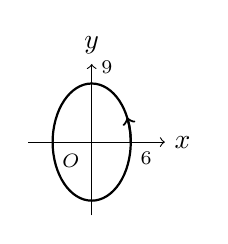
\begin{tikzpicture}[scale=0.62, baseline=(current bounding box.north)]
        \draw[->] (-1.3,0) -- (1.5,0) node[right] {$x$};
        \draw[->] (0,-1.5) -- (0,1.6) node[above] {$y$};
        \draw[thick] (0,0) ellipse (0.8 and 1.2);
        \draw[->, thick] (0.8,0) arc (0:25:0.8 and 1.2);
        \node[below left] at (-0.05,-0.05) {\scriptsize $O$};
        \node[below right] at (0.8,0) {\scriptsize $6$};
        \node[above right] at (0,1.2) {\scriptsize $9$};
    \end{tikzpicture}
    \end{minipage}

    \item $A$ 和 $B$ 两个相同的物体，具有相同的温度，$A$ 周围的温度低于 $A$，而 $B$ 周围的温度高于 $B$，则 $A$、$B$ 二物体在单位时间内辐射的能量 $E(A)$、$E(B)$ 的关系为：\choicebox\\
    (A) $E(A) > E(B)$\qquad (B) $E(A) < E(B)$\qquad (C) $E(A) = E(B)$\qquad (D) 无法判断

    \item 在折射率 $n_3 = 1.60$ 的玻璃片表面镀一层折射率 $n_2 = 1.38$ 的 $\mathrm{MgF_2}$ 薄膜作为增透膜。为了使波长为 $\lambda = 500\ \mathrm{nm}$ 的光，从折射率 $n_1 = 1.00$ 的空气垂直入射到玻璃片上的反射尽可能地减少，$\mathrm{MgF_2}$ 薄膜的厚度 $e$ 至少是\choicebox\\
    (A) $250\ \mathrm{nm}$\qquad (B) $181.2\ \mathrm{nm}$\qquad (C) $125\ \mathrm{nm}$\qquad (D) $90.6\ \mathrm{nm}$

    \item 一平面简谐波在弹性媒质中传播，在媒质质元从最大位移处回到平衡位置的过程中\choicebox\\
    (A) 它的势能转换成动能；\qquad\qquad\qquad (B) 它的动能转换成势能；\\
    (C) 它从相邻的一段媒质质元获得能量，其能量逐渐增加；\\
    (D) 它把自己的能量传给相邻的一段媒质质元，其能量逐渐减小。

    \item 强度为 $I_0$ 的自然光，经过两块互相叠合的偏振片后，光强为 $I_0/8$，则这两块偏振片的偏振化方向夹角是\choicebox\\
    (A) $\pi/3$\qquad (B) $\pi/4$\qquad (C) $\pi/6$\qquad (D) $\pi/2$

    \item \begin{minipage}[t]{0.64\textwidth}
    在如图所示的单缝夫琅禾费衍射实验中，若将单缝沿透镜光轴方向向透镜平移，则屏幕上的衍射条纹\choicebox\\
    (A) 间距变大；\qquad\qquad (B) 间距变小；\\
    (C) 不发生变化；\qquad\quad (D) 间距不变，但明暗条纹的位置交替变化。
    \end{minipage}%
    \begin{minipage}[t]{0.34\textwidth}
    \centering
    \begin{tikzpicture}[scale=0.62, baseline=(current bounding box.north)]
        % 单缝
        \draw[very thick] (0,1.1) -- (0,0.35);
        \draw[very thick] (0,-0.35) -- (0,-1.1);
        \node[above] at (0,1.1) {\scriptsize 单缝};
        % 光轴
        \draw[dashed] (-0.8,0) -- (2.8,0);
        % 入射光
        \draw[->, >=stealth] (-0.9,0.25) -- (0,0.25);
        \draw[->, >=stealth] (-0.9,-0.25) -- (0,-0.25);
        \node[left] at (-0.9,0.25) {\scriptsize $\lambda$};
        % 透镜 L
        \draw[thick] (1.1,-1.0) .. controls (1.35,-0.3) and (1.35,0.3) .. (1.1,1.0);
        \draw[thick] (1.1,-1.0) .. controls (0.85,-0.3) and (0.85,0.3) .. (1.1,1.0);
        \node[above] at (1.1,1.05) {\scriptsize $L$};
        % 屏幕
        \draw[thick] (2.8,-1.1) -- (2.8,1.1);
        \node[above] at (2.8,1.1) {\scriptsize 屏幕};
        % 焦距 f
        \draw[<->, >=stealth, thin] (1.1,-1.15) -- (2.8,-1.15) node[midway, below] {\scriptsize $f$};
    \end{tikzpicture}
    \end{minipage}

    \item 在惯性参考系 $S$ 中，有两个静止质量都是 $m_0$ 的粒子 $A$ 和 $B$，分别以速度 $v$ 沿同一直线相向运动，相碰后合在一起成为一个粒子，则合成粒子静止质量 $M_0$ 的值为（$c$ 表示真空中光速）\choicebox\\
    (A) $2m_0$\qquad (B) $2m_0\sqrt{1-(v/c)^2}$\qquad (C) $\frac{m_0}{2}\sqrt{1-(v/c)^2}$\qquad (D) $\frac{2m_0}{\sqrt{1-(v/c)^2}}$

    \item 一维无限深方势阱中，已知势阱宽度为 $a$。应用不确定关系估计势阱中质量为 $m$ 的粒子的零点能量为\choicebox\\
    (A) $\hbar/(ma^2)$\qquad (B) $\hbar^2/(2ma^2)$\qquad (C) $\hbar^2/(2ma)$\qquad (D) $\hbar/(2ma^2)$

    \item \begin{minipage}[t]{0.66\textwidth}
    一束自然光自空气射向一块平板玻璃（如图），设入射角等于布儒斯特角 $i_0$，则在界面 2 的反射光\choicebox\\
    (A) 是自然光；\\
    (B) 是线偏振光且光矢量的振动方向垂直于入射面；\\
    (C) 是线偏振光且光矢量的振动方向平行于入射面；\\
    (D) 是部分偏振光。
    \end{minipage}%
    \begin{minipage}[t]{0.32\textwidth}
    \centering
    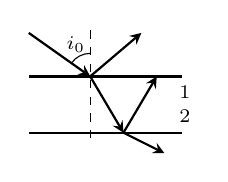
\begin{tikzpicture}[scale=0.65, baseline=(current bounding box.north)]
        % 玻璃板
        \draw[thick] (-1.2,0) -- (1.8,0);
        \draw[thick] (-1.2,-1.1) -- (1.8,-1.1);
        \node[below right] at (1.55,0) {\scriptsize 1};
        \node[above right] at (1.55,-1.1) {\scriptsize 2};
        % 法线
        \draw[dashed] (0,0.9) -- (0,-1.2);
        % 入射光
        \draw[->, >=stealth, thick] (-1.2,0.85) -- (0,0);
        % 入射角 i0
        \draw (0,0.45) arc (90:144:0.45);
        \node at (-0.28,0.62) {\scriptsize $i_0$};
        % 界面1反射光
        \draw[->, >=stealth, thick] (0,0) -- (1.0,0.85);
        % 折射光到界面2
        \draw[->, >=stealth, thick] (0,0) -- (0.65,-1.1);
        % 界面2反射光与折射光
        \draw[->, >=stealth, thick] (0.65,-1.1) -- (1.3,0);
        \draw[->, >=stealth, thick] (0.65,-1.1) -- (1.45,-1.5);
    \end{tikzpicture}
    \end{minipage}
\end{enumerate}

\section*{二、填空题（共 36 分）}

\begin{enumerate}[leftmargin=2em, itemsep=6pt, start=11]
    \item \begin{minipage}[t]{0.68\textwidth}
    在用钠光（$\lambda = 589.3\ \mathrm{nm}$）照亮的缝 $S$ 和双棱镜获得干涉条纹时，将一折射率为 $1.33$ 的平行平面透明膜插入双棱镜上半棱镜的光路中，发现干涉条纹的中心极大（零级）移到原来不放膜时的第五级极大处，则膜厚为\blank[2.8cm]。
    \end{minipage}%
    \begin{minipage}[t]{0.30\textwidth}
    \centering
    \begin{tikzpicture}[scale=0.65, baseline=(current bounding box.north)]
        \draw[dashed] (-1.4,0) -- (1.5,0);
        \fill (-1.2,0) circle (1.5pt) node[above] {\scriptsize $S$};
        % 膜
        \draw[fill=gray!25] (-0.35,0.08) rectangle (-0.23,0.95);
        \node[left] at (-0.35,0.75) {\scriptsize 膜};
        % 双棱镜
        \draw[thick] (0.2,-0.95) -- (0.2,0.95) -- (0.55,0) -- cycle;
        \draw[thick] (0.2,0) -- (0.55,0);
    \end{tikzpicture}
    \end{minipage}

    \item \begin{minipage}[t]{0.68\textwidth}
    设沿弦线传播的一入射波的表达式是 $y_1 = A\cos\left[2\pi\left(\nu t - \frac{x}{\lambda}\right) + \phi\right]$，在 $x=L$ 处（$B$ 点）发生反射，反射点为固定端（如图）。设波在传播和反射过程中振幅不变，则弦线上形成的驻波的表达式为 $y = \blank[5.5cm]$。
    \end{minipage}%
    \begin{minipage}[t]{0.30\textwidth}
    \centering
    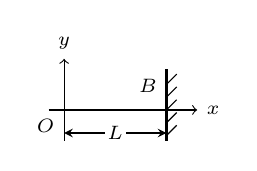
\begin{tikzpicture}[scale=0.65, baseline=(current bounding box.north)]
        \draw[->] (-0.3,0) -- (2.6,0) node[right] {\scriptsize $x$};
        \draw[->] (0,-0.6) -- (0,1.0) node[above] {\scriptsize $y$};
        \node[below left] at (0,0) {\scriptsize $O$};
        \draw[very thick] (2.0,-0.6) -- (2.0,0.8);
        \foreach \y in {-0.5,-0.25,0,0.25,0.5} {\draw (2.0,\y) -- (2.2,\y+0.2);}
        \node[above left] at (2.0,0.15) {\scriptsize $B$};
        \draw[<->, >=stealth, thin] (0,-0.45) -- (2.0,-0.45) node[midway, fill=white, inner sep=1pt] {\scriptsize $L$};
    \end{tikzpicture}
    \end{minipage}

    \item 一物体作简谐振动，周期为 $T$，求在第一个周期内经过：（1）由平衡位置到位移最大处所需的时间为\blank[2.0cm]；（2）由平衡位置到位移最大处的 $1/2$ 处所需的时间为\blank[2.0cm]。

    \item 一质量为 $m$ 的小球在一个光滑的半径为 $R$ 的球形碗底作微小振动。设 $t=0$ 时，$\theta=0$，小球的速度为 $v_0$，并向右运动。求在振幅很小的情况下，小球的运动方程为\blank[4.0cm]。

    \item 已知有两谐振动在同一方向上运动，方程为 $x_1 = 5\cos(10t + 0.75\pi)\ \mathrm{cm}$，$x_2 = 6\cos(10t + 0.25\pi)\ \mathrm{cm}$，则合振动的振幅为\blank[2.5cm]。

    \item 用牛顿环实验测单色光波长。当用已知波长为 $\lambda = 589.3\ \mathrm{nm}$ 的光垂直照射时，测得第一级和第四级暗环的距离 $\Delta_1 = 4.00\times 10^{-3}\ \mathrm{m}$；当用未知的单色光垂直照射时，测得第一级和第四级暗环的距离 $\Delta_2 = 3.85\times 10^{-3}\ \mathrm{m}$，则未知单色光的波长是\blank[2.2cm]$\mathrm{nm}$。

    \item 一驻波方程为 $y = 0.5\cos\frac{\pi x}{3}\cos 40\pi t\ (x,y:\mathrm{cm};\ t:\mathrm{s})$，则形成驻波的两成分波的振幅为\blank[1.8cm]；周期为\blank[1.8cm]；波速为\blank[2.0cm]；该驻波的两相邻波节之间距离为\blank[1.8cm]。

    \item 波长 $\lambda = 600.0\ \mathrm{nm}$ 的单色光垂直入射在光栅上，光栅常数 $d=3600\ \mathrm{nm}$，则第三级明条纹的衍射角为\blank[1.8cm]；欲使该条纹的衍射角为 $45^\circ$，则入射角应变为\blank[2.0cm]；入射角与衍射角应在光栅平面法线\blank[1.5cm]（同或异）侧。

    \item 普朗克的量子假说是为了解释\blank[3.0cm]的实验规律而提出来的。

    \item 一宇宙飞船以 $c/2$（$c$ 为真空中的光速）的速率相对地面运动。从飞船中以相对飞船为 $c/2$ 的速率向前发射一枚火箭，假设发射火箭不影响飞船原有速率，则地面上的观察者测得火箭的速率为\blank[2.5cm]。

    \item 电子的静止质量为 $m_0$，若以速度 $v = 0.6c$ 运动，则它的德布罗意波长为\blank[2.5cm]，频率为\blank[2.5cm]。
\end{enumerate}

\section*{三、计算题（共 34 分）}

\begin{enumerate}[leftmargin=2em, itemsep=8pt, start=22]
    \item \begin{minipage}[t]{0.68\textwidth}
    （10 分）如图所示，水平轻质弹簧一端固定，另一端所系轻绳绕过一滑轮垂挂一质量为 $m$ 的物体。若弹簧劲度系数为 $k$，滑轮半径为 $R$，转动惯量为 $J$。（1）证明物体作简谐振动；（2）求振动周期；（3）设 $t=0$ 时弹簧无伸缩，物体由静止下落，写出物体的运动方程。
    \end{minipage}%
    \begin{minipage}[t]{0.30\textwidth}
    \centering
    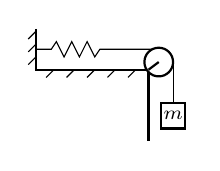
\begin{tikzpicture}[scale=0.65, baseline=(current bounding box.north)]
        % 墙面与桌面
        \draw[thick] (0,0.6) -- (0,-0.2) -- (2.2,-0.2) -- (2.2,-1.6);
        \foreach \y in {-0.1,0.15,0.4} {\draw (-0.15,\y) -- (0,\y+0.15);}
        \foreach \x in {0.2,0.6,1.0,1.4,1.8} {\draw (\x,-0.35) -- (\x+0.15,-0.2);}
        % 弹簧
        \draw (0,0.2) -- (0.3,0.2) -- (0.4,0.35) -- (0.55,0.05) -- (0.7,0.35) -- (0.85,0.05) -- (1.0,0.35) -- (1.15,0.05) -- (1.25,0.2) -- (2.4,0.2);
        % 滑轮
        \draw[thick, fill=white] (2.4,-0.05) circle (0.28);
        \draw[thick] (2.2,-0.2) -- (2.4,-0.05);
        % 绳与重物 m
        \draw (2.68,-0.05) -- (2.68,-0.85);
        \draw[thick] (2.45,-0.85) rectangle (2.91,-1.35);
        \node at (2.68,-1.1) {\scriptsize $m$};
    \end{tikzpicture}
    \end{minipage}

    \item （6 分）图表示两个同方向、同频率的简谐振动曲线，其角频率为 $\omega$，分别求出（a）和（b）情形时：（1）合振动振幅；（2）合振动的振动方程。
    \begin{center}
    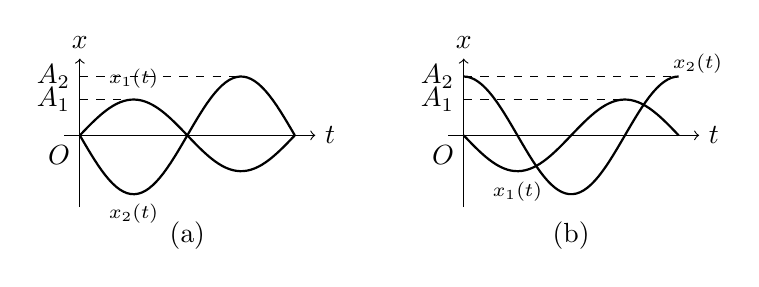
\begin{tikzpicture}[scale=0.65]
        % (a)
        \begin{scope}
            \draw[->] (-0.3,0) -- (4.6,0) node[right] {$t$};
            \draw[->] (0,-1.4) -- (0,1.5) node[above] {$x$};
            \draw[thick, domain=0:4.2, samples=60] plot (\x, {0.7*sin(180*\x/2.1)});
            \draw[thick, domain=0:4.2, samples=60] plot (\x, {-1.15*sin(180*\x/2.1)});
            \draw[dashed] (0,0.7) node[left] {$A_1$} -- (1.05,0.7);
            \draw[dashed] (0,1.15) node[left] {$A_2$} -- (3.15,1.15);
            \node[below left] at (0,0) {$O$};
            \node[above] at (1.05,0.72) {\scriptsize $x_1(t)$};
            \node[below] at (1.05,-1.15) {\scriptsize $x_2(t)$};
            \node[below] at (2.1,-1.5) {(a)};
        \end{scope}
        % (b)
        \begin{scope}[xshift=7.5cm]
            \draw[->] (-0.3,0) -- (4.6,0) node[right] {$t$};
            \draw[->] (0,-1.4) -- (0,1.5) node[above] {$x$};
            \draw[thick, domain=0:4.2, samples=60] plot (\x, {-0.7*sin(180*\x/2.1)});
            \draw[thick, domain=0:4.2, samples=60] plot (\x, {1.15*cos(180*\x/2.1)});
            \draw[dashed] (0,0.7) node[left] {$A_1$} -- (3.15,0.7);
            \draw[dashed] (0,1.15) node[left] {$A_2$} -- (4.2,1.15);
            \node[below left] at (0,0) {$O$};
            \node[below] at (1.05,-0.72) {\scriptsize $x_1(t)$};
            \node[above right] at (3.9,1.02) {\scriptsize $x_2(t)$};
            \node[below] at (2.1,-1.5) {(b)};
        \end{scope}
    \end{tikzpicture}
    \end{center}

    \item （7 分）有一单缝，缝宽 $a=0.60\ \mathrm{mm}$，缝后放一焦距 $f=400\ \mathrm{mm}$ 的透镜，现用一束白光（$400\sim 760\ \mathrm{nm}$）垂直入射，并在焦面处的屏幕上形成衍射条纹。求：\\
    （1）哪些波长的光在离中心点 $x=1.4\ \mathrm{mm}$ 处的 $P$ 点形成亮纹；\\
    （2）它们在 $P$ 点产生亮纹的级次；\\
    （3）从 $P$ 点看来，该狭缝对这些波长可分成的半波带数。

    \item （6 分）在白光下，观察一层置于空气中的折射率为 $1.30$ 的薄油膜，若观察方向与油膜表面法线成 $30^\circ$ 角时，可看到油膜呈蓝色（波长为 $480\ \mathrm{nm}$），试求油膜的最小厚度。如果从法向观察，反射光呈什么颜色？

    \item （5 分）一个电子的动能等于它的静能，试求该电子的速率和德布罗意波长。
\end{enumerate}

\end{document}
